\documentclass[journal, 12pt, twocolumn]{IEEEtran}
\usepackage[utf8]{inputenc}
\usepackage{graphicx}
\usepackage{amssymb}
\usepackage{amsmath}
\graphicspath{{figs/}}
\title{AI1110 Assignment 1}
\author{Abhinav Yadav, cs21btech11002}

\begin{document}
    \maketitle

    \textbf{ICSE class 10 paper 2019}\\
    \textbf{Q11 (b):}
    The product of two consecutive natural numbers which are multiples of 3 is 
    equal to 810. Find the two numbers.\\\\
    \textbf{Solution:}\\
    Let the two consecutive natural numbers which are multiples of $3$ be $3n$ and $3n+3$
    \hspace{5pt} $\exists \hspace{2pt} n \in \mathbb{N}$\\\\
    \textbf{According to the question:}
    \begin{align}
        &&3n(3n+3) &= 810\\
        &\implies & 9n(n+1) &= 810\\
        &\implies & n(n+1) &= 90\\
        &\implies & n^2+n-90 &= 0\hspace{25pt}\\
        &\implies & (n+10)(n-9) &= 0\\
        &\implies & n=-10 \hspace{15pt} &or \hspace{15pt} n=9
        \intertext{discarding $n=-10$ as $n \in \mathbb{N}$}
        &\implies & n &= 9\\
        &\implies & 3n &= 27\\
        &\implies & 3n+3 &= 30
    \end{align}
    The two numbers are:\vspace{200pt}
    \fbox{$27, 30$}\pagebreak

    Plot of $eq^n(4)$ is:
    \begin{figure}[h]
        \centering
        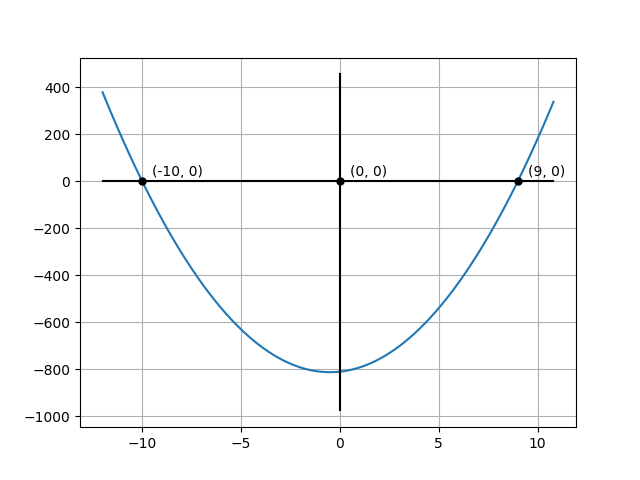
\includegraphics[width=\columnwidth]{plot.png}
        \caption{Plot showing the polynomial in $eq^n(4)$}
        \label{Fig1}
    \end{figure}\\
    It can be easily verified by observing the plot that the roots of $eq^n (4)$ are 9 and -10.\\\\

    The output of the program used to find and verify these numbers is:
    \begin{figure}[h]
        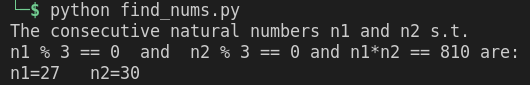
\includegraphics[width=\columnwidth]{output.png}
        \caption{Output of the python program}
    \end{figure}
\end{document}